\chapter{Projects --- プロジェクトの進捗を可視化する}

\section{この章で学ぶこと}

ソフトウェア開発では、コードを書くことと同じくらい「何を、いつ、誰が作るか」を管理することが重要です。タスクの優先順位、進捗状況、期限、担当者といった情報が整理されていないと、チームは迷走してしまいます。

これまで多くのチームが、Trello、Jira、Asanaといった外部のプロジェクト管理ツールを使ってきました。しかし、外部ツールを使うと、GitHubのIssueやPull Requestとの連携が煩雑になりがちです。「Jiraのチケットを更新して、GitHubのIssueも更新して...」という二重管理は、開発者の負担を増やします。

\textbf{GitHub Projects}は、この問題を解決するためにGitHubが提供するプロジェクト管理機能です。IssueやPull Requestと完全に統合されているため、開発の流れから離れることなくタスクの管理ができます。

この章を読み終えると、以下のことができるようになります。

\begin{itemize}
  \item GitHub Projectsの位置づけと特徴を理解する
  \item Board、Table、Roadmapの3つのビューを使い分けられる
  \item カスタムフィールドを定義してプロジェクトに合った管理体制を構築できる
  \item ワークフロー自動化を設定して手作業を減らせる
  \item Organizationレベルのプロジェクトで複数リポジトリを横断的に管理できる
\end{itemize}

\section{GitHub Projectsとは}

\subsection{プロジェクト管理ツールとしての位置づけ}

GitHub Projectsは、GitHubに内蔵されたプロジェクト管理ツールです。以前は「Projects（Classic）」と呼ばれるシンプルなカンバンボード機能がありましたが、現在の「Projects」はそれを大幅に進化させた新しいバージョンです。

GitHub Projectsの最大の特徴は、\textbf{IssueやPull Requestとのネイティブな統合}です。Projectのアイテムは、既存のIssueやPull Requestそのものです。Issueのステータスを変更すればProjectのボードに反映され、Pull Requestがマージされれば自動的にタスクが完了になる、といった連携が自然に行えます。

もうひとつの重要な特徴は、\textbf{柔軟なビューとカスタマイズ性}です。同じデータをカンバンボード、スプレッドシート、タイムラインなど複数の形式で表示でき、プロジェクトの状況をさまざまな角度から把握できます。

GitHub Projectsを使うべき場面と、外部ツールを検討すべき場面を整理しておきましょう。GitHubでコードを管理しているチームで、Issueベースのタスクをシンプルに追跡したい場合は、GitHub Projectsが最適です。一方、大規模なエンタープライズで高度なレポーティングやリソース管理が必要な場合は、Jiraのような専門ツールの方が適しているかもしれません。

\section{Projectの作成}

\subsection{作成手順}

Projectの作成は、GitHubのWebインターフェースから行います。

\begin{enumerate}
  \item GitHubの右上にあるプロフィールアイコンをクリックし、「\textbf{Your projects}」を選択します
  \item 「\textbf{New project}」ボタンをクリックします
  \item テンプレートを選択します。いくつかのプリセットテンプレートが用意されていますが、「\textbf{Board}」「\textbf{Table}」「\textbf{Roadmap}」から選ぶのが基本です。白紙から始めたい場合は空のテンプレートを選びます
  \item プロジェクト名を入力し、「\textbf{Create project}」をクリックします
\end{enumerate}

\begin{figure}[htbp]
\centering
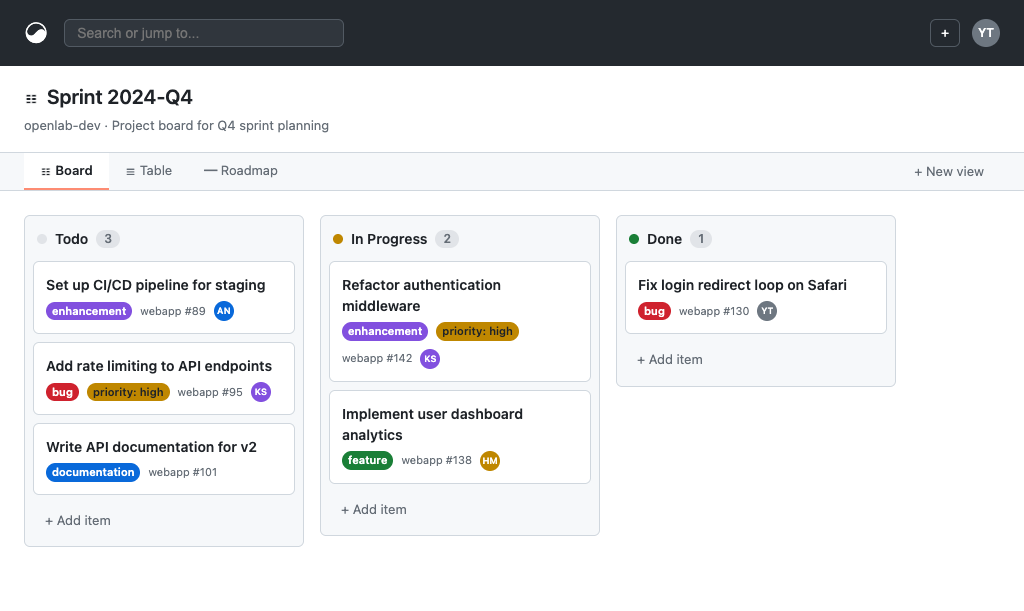
\includegraphics[width=0.95\textwidth]{images/projects-board.png}
\caption{Projectの新規作成画面でテンプレートを選択する様子}
\end{figure}

Projectが作成されたら、既存のIssueやPull Requestをアイテムとして追加できます。CLI からも操作できます。

\begin{lstlisting}[language=bash]
# ProjectにIssueを追加
gh project item-add PROJECT_NUMBER --owner USERNAME \
  --url https://github.com/owner/repo/issues/42
\end{lstlisting}

ボード上で「\textbf{+}」ボタンをクリックすると、\textbf{ドラフトアイテム}を直接作成することもできます。ドラフトアイテムはまだIssueになっていない簡易的なメモのようなもので、後からIssueに変換できます。アイデアを素早くメモしておきたいときに便利です。

\subsection{3つのビュー}

GitHub Projectsでは、同じデータを異なるビューで表示できます。それぞれのビューには得意とする場面があり、プロジェクトの状況に応じて使い分けることが重要です。

\subsubsection{Board（ボード）ビュー}

Boardビューは、いわゆる\textbf{カンバンボード}です。アイテムがカード形式で表示され、ステータスごとの列（カラム）に分類されます。典型的な列の構成は「Todo」「In Progress」「Done」の3列ですが、プロジェクトに応じて自由にカスタマイズできます。

\begin{figure}[htbp]
\centering
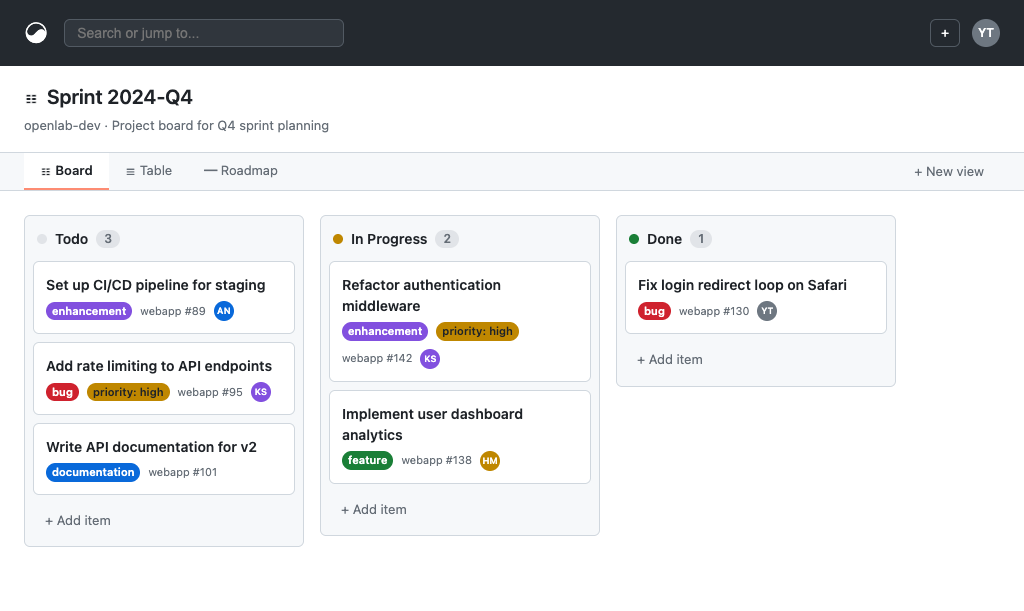
\includegraphics[width=0.95\textwidth]{images/projects-board.png}
\caption{Boardビューのカンバンボード}
\end{figure}

Boardビューの利点は、\textbf{進捗状況が一目で分かる}ことです。「In Progress」の列にカードが溜まりすぎていれば、チームが多くのタスクを同時に抱えすぎていることが分かります。カードをドラッグ\&ドロップで別の列に移動でき、直感的な操作が可能です。

Boardビューは、日々の開発作業の管理、スプリントの進捗確認、チームのデイリースタンドアップミーティングでの状況共有などに適しています。

\subsubsection{Table（テーブル）ビュー}

Tableビューは、\textbf{スプレッドシートのような表形式}でアイテムを表示します。各列にカスタムフィールド（後述）を配置でき、データの並べ替えやフィルタリングが自在にできます。

\begin{figure}[htbp]
\centering
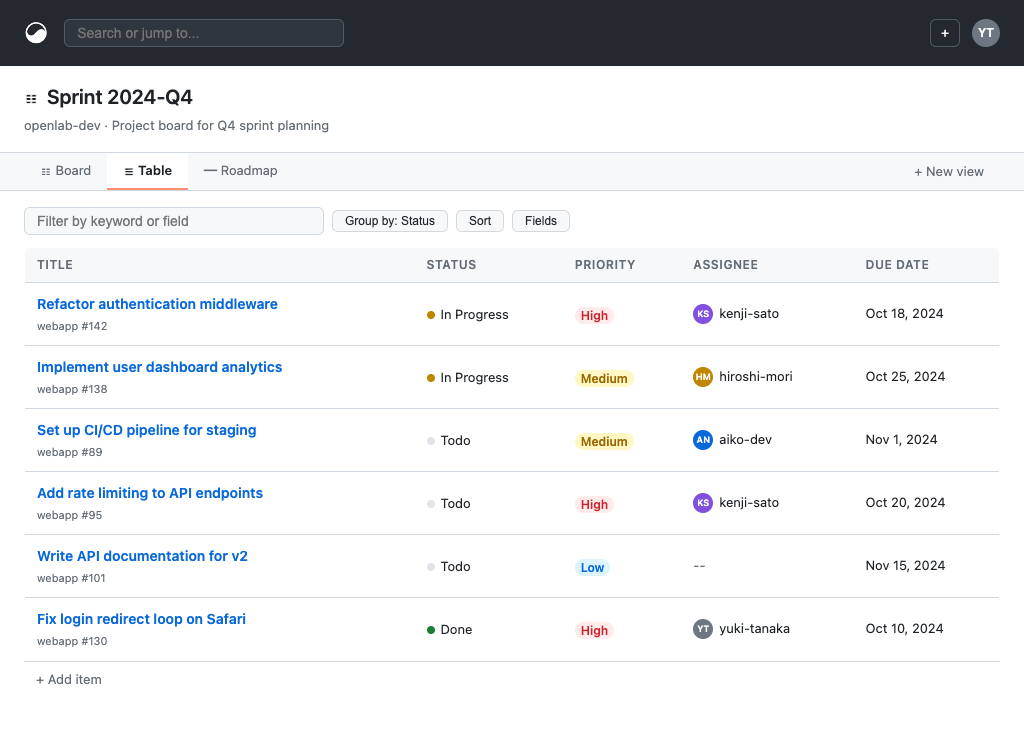
\includegraphics[width=0.95\textwidth]{images/projects-table.png}
\caption{Tableビューのスプレッドシート風表示}
\end{figure}

Tableビューの利点は、\textbf{大量のアイテムを効率的に一覧・編集できる}ことです。優先度、見積もりポイント、期限、担当者など、複数の情報を同時に確認・編集できます。また、列ヘッダーをクリックして並べ替えたり、フィルターを適用して特定の条件のアイテムだけを表示したりできます。

Tableビューは、バックログの管理、スプリントプランニング、プロジェクト全体のタスク一覧の俯瞰などに適しています。

\subsubsection{Roadmap（ロードマップ）ビュー}

Roadmapビューは、\textbf{タイムライン形式（ガントチャート風）}でアイテムを時系列に表示します。このビューを使うには、アイテムに日付フィールド（開始日や期限）が設定されている必要があります。

\begin{figure}[htbp]
\centering
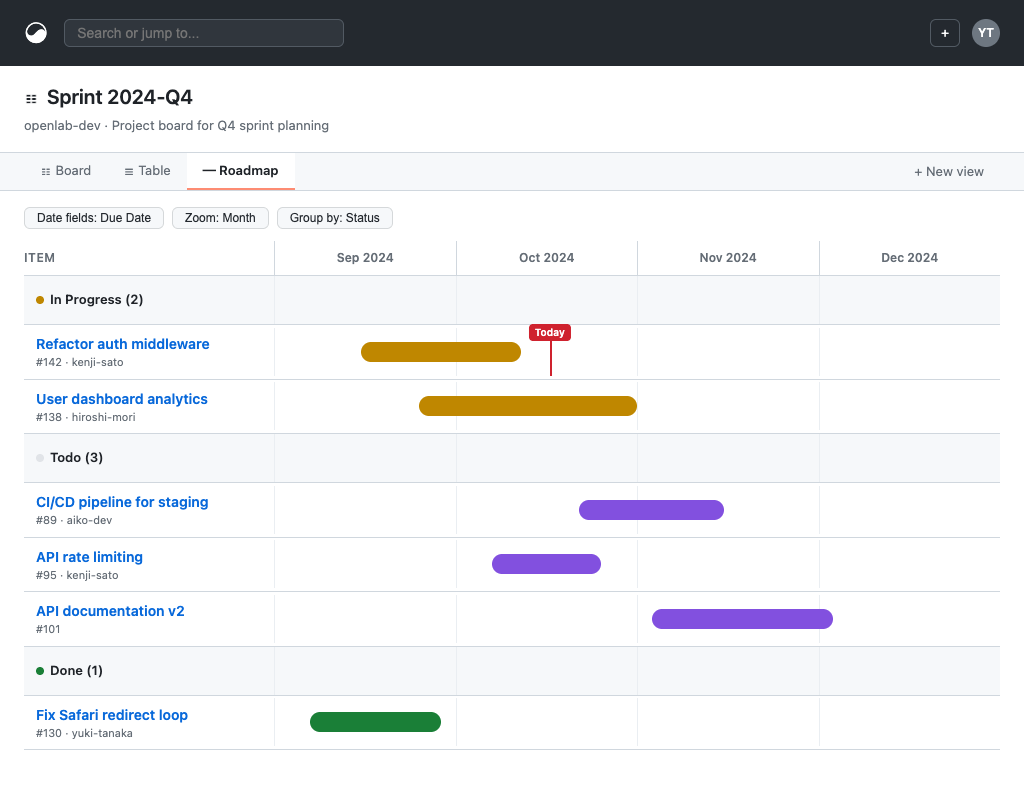
\includegraphics[width=0.95\textwidth]{images/projects-roadmap.png}
\caption{Roadmapビューのタイムライン表示}
\end{figure}

Roadmapビューの利点は、\textbf{時間軸に沿った計画と進捗が視覚的に分かる}ことです。各タスクがいつ開始され、いつ完了予定かをバーの長さで表現するため、スケジュールの重なりや遅延が一目で把握できます。

Roadmapビューは、中長期的なプロジェクト計画の共有、マイルストーンの管理、ステークホルダーへの報告などに適しています。

\subsection{複数のビューを組み合わせる}

ひとつのProjectに対して、複数のビューを作成できます。たとえば、「開発チーム用のBoardビュー」「プロジェクトマネージャー用のTableビュー」「経営層向けのRoadmapビュー」を同じProjectに用意しておけば、同じデータを異なる視点から確認できます。

ビューの追加は、Projectのタブの右端にある「\textbf{+}」ボタンから行えます。各ビューには独立したフィルターやソート設定を保存できるため、用途に応じた表示をいつでも切り替えられます。

\section{カスタムフィールド}

GitHub Projectsでは、プロジェクトの管理に必要な情報を\textbf{カスタムフィールド}として定義できます。デフォルトで用意されている「Title」「Assignees」「Status」に加えて、プロジェクト固有の情報を追加することで、より効果的な管理が可能になります。

カスタムフィールドの追加は、Tableビューの列ヘッダーの右端にある「\textbf{+}」ボタンから行います。以下の型が利用できます。

\subsection{Text（テキスト）}

自由記述のテキストフィールドです。メモ、関連するドキュメントのURL、設計上の注意点など、定型化しにくい情報を記録するのに適しています。

使用例：参照ドキュメントのURL、技術的な補足メモ

\subsection{Number（数値）}

数値を入力するフィールドです。ストーリーポイント（タスクの相対的な作業量を表す指標）、見積もり時間、優先度のスコアなどに使います。Tableビューでは、Number フィールドの合計値を表示することもでき、スプリント全体の作業量を把握するのに役立ちます。

使用例：ストーリーポイント（1, 2, 3, 5, 8, 13）、見積もり工数（時間）

\subsection{Date（日付）}

日付を入力するフィールドです。タスクの開始日、期限（デッドライン）、実際の完了日などを記録します。Roadmapビューを使う場合、Dateフィールドは必須です。開始日と終了日の2つのDateフィールドを設定すると、Roadmapビューでタスクの期間がバーとして表示されます。

使用例：開始予定日、期限、実際の完了日

\subsection{Single select（単一選択）}

あらかじめ定義した選択肢の中から1つを選ぶフィールドです。優先度（High / Medium / Low）、カテゴリ（Bug / Feature / Improvement）、担当チーム（Frontend / Backend / DevOps）など、分類に使うフィールドに最適です。各選択肢には色を設定できるため、視覚的にも分かりやすい管理が可能です。

使用例：
\begin{itemize}
  \item 優先度：\cmd{Critical}（赤）、\cmd{High}（オレンジ）、\cmd{Medium}（黄）、\cmd{Low}（青）
  \item カテゴリ：\cmd{Bug}（赤）、\cmd{Feature}（緑）、\cmd{Documentation}（紫）
\end{itemize}

\subsection{Iteration（イテレーション）}

スプリントやイテレーションを管理するための特別なフィールドです。開始日と期間（通常1〜4週間）を設定すると、自動的にイテレーションの区切りが生成されます。アジャイル開発で「Sprint 1」「Sprint 2」のようにタスクを区切って管理する場合に便利です。

Iterationフィールドを使うと、Boardビューでイテレーションごとにグループ化して表示したり、Tableビューで特定のイテレーションのタスクだけをフィルタリングしたりできます。

使用例：2週間スプリント（Sprint 1: 4/1〜4/14、Sprint 2: 4/15〜4/28）

\begin{figure}[htbp]
\centering
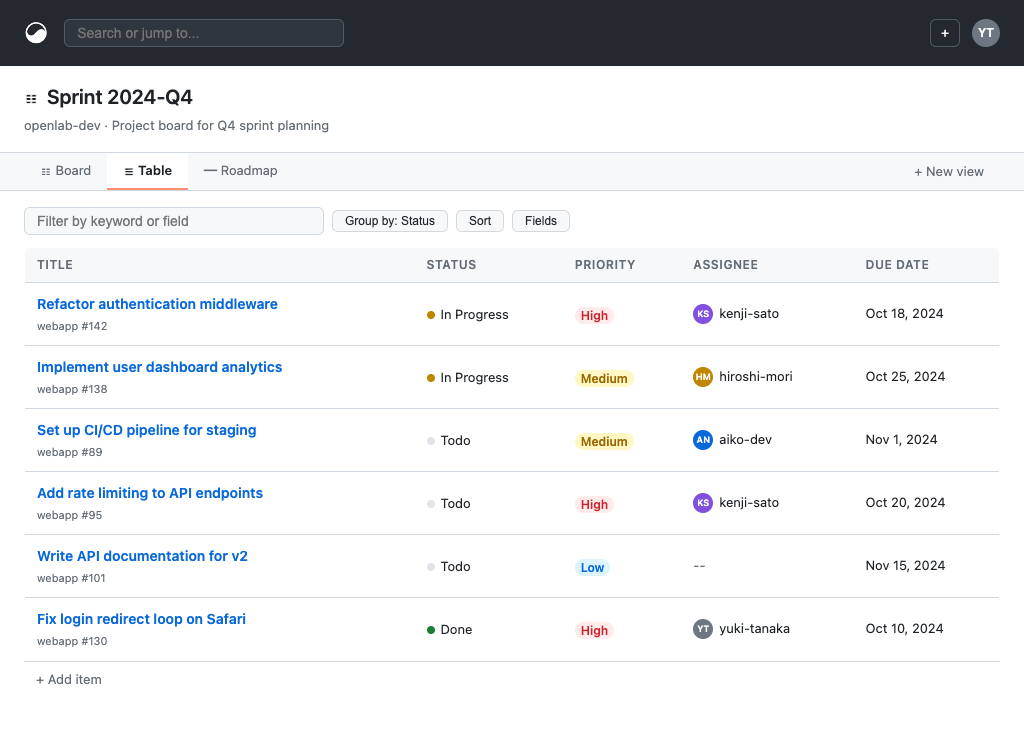
\includegraphics[width=0.95\textwidth]{images/projects-table.png}
\caption{カスタムフィールドの設定画面}
\end{figure}

\subsection{フィールド設計のヒント}

カスタムフィールドは多すぎるとかえって管理の負担が増えます。最初は必要最小限のフィールドから始めて、チームの運用を見ながら徐々に追加していくことをお勧めします。以下は、小〜中規模のプロジェクトにおける基本的なフィールド構成の例です。

\begin{tabular}{|l|l|l|}
\hline
\textbf{フィールド名} & \textbf{型} & \textbf{用途} \\
\hline
Status & Single select & Todo / In Progress / In Review / Done \\
\hline
Priority & Single select & High / Medium / Low \\
\hline
Sprint & Iteration & 2週間ごとのスプリント \\
\hline
Story Points & Number & タスクの相対的な作業量 \\
\hline
Due Date & Date & タスクの期限 \\
\hline
\end{tabular}

\section{ワークフロー自動化}

プロジェクト管理で最も面倒なのは、ステータスの手動更新です。Issueがクローズされたら「Done」に移動する、Pull Requestがマージされたらタスクを完了にするといった操作を毎回手動で行うのは、忘れがちですし時間の無駄です。

GitHub Projectsの\textbf{ワークフロー自動化}機能を使えば、特定のイベントが発生したときにアイテムのステータスを自動的に変更できます。

\subsection{設定方法}

ワークフローの設定は、Projectの設定画面から行います。

\begin{enumerate}
  \item Projectのページを開きます
  \item 右上の「\textbf{...}」メニュー（または設定アイコン）をクリックし、「\textbf{Workflows}」を選択します
  \item 利用可能なワークフローの一覧が表示されます
  \item 有効にしたいワークフローのトグルをオンにし、条件と動作を設定します
\end{enumerate}

\begin{figure}[htbp]
\centering
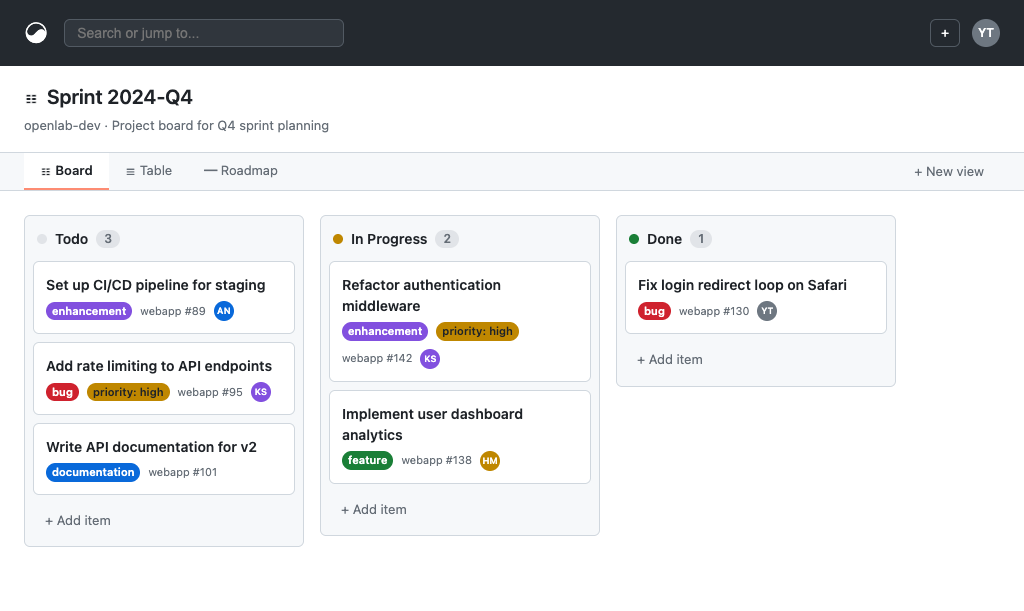
\includegraphics[width=0.95\textwidth]{images/projects-board.png}
\caption{ワークフロー設定画面}
\end{figure}

\subsection{主なワークフロー}

\textbf{Item added to project（アイテム追加時）}は、IssueやPull RequestがProjectに追加されたときに発動するワークフローです。新しいアイテムが追加されたら自動的にステータスを「Todo」に設定する、といった使い方が一般的です。これにより、追加されたアイテムがステータスなしの状態で放置されることを防げます。

\textbf{Item closed（アイテムクローズ時）}は、IssueがクローズされたときにProjectのステータスを自動更新するワークフローです。たとえば、Issueがクローズされたら自動的にステータスを「Done」に変更する設定にしておけば、手動でカードを移動する手間が省けます。

\textbf{Pull request merged（PRマージ時）}は、Pull Requestがマージされたときに発動するワークフローです。マージされたらステータスを「Done」に変更する設定が典型的です。\cmd{Closes \#42}のようにPRとIssueが紐付いている場合、PRのマージによってIssueもクローズされ、両方が「Done」になります。

\textbf{Item reopened（アイテム再オープン時）}は、一度クローズされたIssueが再オープンされたときに、ステータスを「In Progress」や「Todo」に戻すワークフローです。

これらのワークフローを適切に設定しておくと、チームメンバーは日常的にIssueのオープン・クローズやPull Requestのマージだけに集中すれば、Projectのボードが自動的に最新の状態に保たれます。

\subsection{より高度な自動化}

組み込みのワークフロー以外にも、GitHub Actionsを使ってさらに高度な自動化を実現できます。たとえば、特定のラベルが付けられたIssueを自動的にProjectに追加する、担当者がアサインされたら自動的にステータスを「In Progress」に変更する、といったカスタムワークフローを構築できます。第12章で学んだGitHub Actionsの知識が、ここでも活きてきます。

\section{フィルタリングとソート}

Projectに多くのアイテムが登録されてくると、必要な情報を素早く見つけるためのフィルタリングとソートが重要になります。GitHub Projectsでは、ビューごとに独立したフィルターとソート条件を設定・保存できます。

\subsection{フィルタの記法}

フィルターバーに以下のような構文で条件を入力します。

\begin{lstlisting}[language={}]
# ステータスが「Todo」のアイテムだけ表示
status:Todo

# 自分にアサインされたアイテムだけ表示
assignee:@me

# 特定のラベルが付いたアイテムだけ表示
label:bug

# 優先度が「High」のアイテムだけ表示
priority:High

# 複数の条件を組み合わせる（AND条件）
status:Todo,In Progress assignee:@me label:bug

# 否定条件（特定のステータスを除外）
-status:Done
\end{lstlisting}

複数の値をカンマで区切ると「OR条件」として扱われます。\cmd{status:Todo,In Progress}は「TodoまたはIn Progressのアイテム」を意味します。スペースで区切った複数のフィルターは「AND条件」として扱われます。

\subsection{ソート}

Tableビューでは、列ヘッダーをクリックすることでその列の値に基づいてソートできます。昇順・降順を切り替えることも可能です。複数の列でソートしたい場合は、ビューの設定から詳細なソート条件を指定できます。

たとえば、「優先度の高い順に並べた上で、同じ優先度のアイテムは期限の早い順に並べる」といった複合的なソートが可能です。

\subsection{ビューの保存}

フィルターやソートの設定は、ビューごとに保存できます。日常的に使うフィルター条件は、専用のビューとして保存しておくと便利です。たとえば：

\begin{itemize}
  \item 「マイタスク」ビュー：\cmd{assignee:@me -status:Done} でフィルタリング
  \item 「今週の優先タスク」ビュー：\cmd{status:Todo,In Progress priority:High} でフィルタリング
  \item 「バグ一覧」ビュー：\cmd{label:bug -status:Done} でフィルタリング
\end{itemize}

これらのビューをタブとして並べておけば、ワンクリックで見たい情報に切り替えられます。

\subsection{グループ化}

Boardビューだけでなく、Tableビューでもアイテムをグループ化して表示できます。たとえば、担当者ごとにグループ化すれば「各メンバーがどれだけのタスクを抱えているか」が一目で分かります。スプリントごとにグループ化すれば「各スプリントにどれだけのタスクが割り当てられているか」を確認できます。

\section{Organizationレベルのプロジェクト}

\subsection{複数リポジトリにまたがるプロジェクト管理}

実際の開発では、ひとつのプロダクトが複数のリポジトリにまたがることが珍しくありません。たとえば、フロントエンドのリポジトリ、バックエンドAPIのリポジトリ、インフラ設定のリポジトリが分かれているケースです。それぞれのリポジトリにProjectを作成すると、プロジェクト全体の進捗を把握するのが困難になります。

\textbf{Organizationレベルのプロジェクト}は、この問題を解決します。Organizationに紐付いたProjectを作成すれば、そのOrganization配下の複数のリポジトリのIssueやPull Requestをひとつのボードで一元管理できます。

\begin{figure}[htbp]
\centering
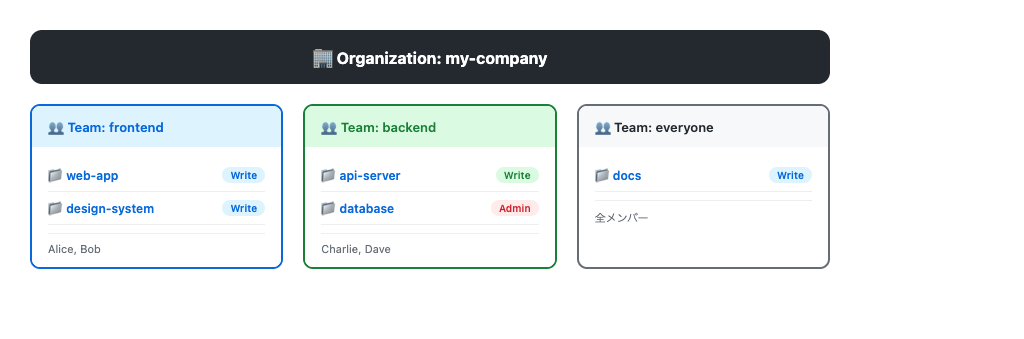
\includegraphics[width=0.9\textwidth]{images/diagram-org-structure.png}
\end{figure}

\subsection{Organizationプロジェクトの作成}

Organizationレベルのプロジェクトを作成するには、Organizationのページから操作します。

\begin{enumerate}
  \item Organizationのページを開きます
  \item \textbf{Projects}タブをクリックします
  \item 「\textbf{New project}」をクリックし、通常のProject作成と同じ手順で作成します
\end{enumerate}

このProjectには、Organizationが所有する任意のリポジトリのIssueやPull Requestを追加できます。あるリポジトリのIssue画面から直接Projectに追加することも、Projectの画面からURLを指定して追加することもできます。

\subsection{実践的な活用パターン}

Organizationプロジェクトの活用パターンをいくつか紹介します。

\textbf{プロダクト単位のプロジェクト}は、ひとつのプロダクトに関わるすべてのリポジトリのタスクを集約します。プロダクトマネージャーがプロダクト全体の進捗を把握するのに適しています。

\textbf{四半期目標のプロジェクト}は、Q1、Q2のように四半期ごとのプロジェクトを作成し、その期間に達成すべきタスクを管理します。期間が終わったらプロジェクトをアーカイブし、新しい四半期のプロジェクトを作成します。

\textbf{チーム横断のプロジェクト}は、複数のチームが協力して進めるプロジェクト（たとえば、大規模なリファクタリングやセキュリティ対応）を管理するのに適しています。各チームのリポジトリからIssueを集め、全体の進捗を可視化します。

\section{まとめ}

この章では、GitHub Projectsを使ったプロジェクト管理の方法について学びました。重要なポイントを振り返りましょう。

\begin{itemize}
  \item \textbf{GitHub Projects}は、IssueやPull Requestと統合されたプロジェクト管理ツールであり、外部ツールとの二重管理を解消できる
  \item \textbf{Board（カンバン）、Table（表形式）、Roadmap（タイムライン）}の3つのビューを目的に応じて使い分ける
  \item \textbf{カスタムフィールド}（Text、Number、Date、Single select、Iteration）を定義して、プロジェクト固有の情報を管理する
  \item \textbf{ワークフロー自動化}を設定すると、Issueのクローズ時やPRのマージ時にステータスが自動更新され、手動管理の手間が省ける
  \item フィルタリング、ソート、グループ化を活用して、大量のアイテムから必要な情報を素早く見つける
  \item \textbf{Organizationレベルのプロジェクト}を使えば、複数リポジトリのIssueを1つのボードで横断的に管理できる
\end{itemize}

GitHub Projectsは、小さなプロジェクトではシンプルなカンバンボードとして、大きなプロジェクトではカスタムフィールドやワークフロー自動化を駆使した高度な管理ツールとして、柔軟に活用できます。まずはシンプルなBoardビューから始めて、チームの運用に合わせて徐々にカスタマイズしていくことをお勧めします。
